%
% 25 Oct 01 - Brian: Added description of endianness analysis during
%              type analysis.
%

\chapter{Type Recovery Analysis}
\label{ch-type}

\newtheorem{typerule}{Type Rule}[chapter]

{\small
\begin{flushright}
Design: Cristina [Mar 99], Implementation: Mike Van Emmerik[c.00], Bernard Wong [Aug 01], Documentation: Cristina [99], Bernard [Aug 01], Brian [Oct 01]
\end{flushright}
}

{\em The bulk of this document was written in 1999 and has not 
been updated much since.  In summer 2001, Bernard implemented some 
of the type propagation ideas presented in this chapter, 
however, the implementation is not fully tested at the 
time of release of this code.} 

Low-level type recovery is the process of recoverying types 
that are available at the machine level in order for 
translated programs to be correct.  
Type recovery is done in a series of steps, by first annotating
locations with their plausible type and then propagating 
types across live ranges of locations.  

This document will grow as we learn more about the type 
requirements for translated programs.  The following are 
the issues that will be addressed throughout this process: 
\begin{itemize}
\item What is the minimal set of low-level types required?
\item How do we best propagate information across procedures?
\item What information do we need to store for byte swapping 
	to work correctly across different endianness machines?
\end{itemize}

In reality, we are mainly interested in determining the low-level 
types for parameters and return values, however, in order to 
do that, one needs to also know the types for other locations 
that define the variables that get passed as parameters. 
This analysis will be done in the following stages: 
\begin{itemize}
\item Recovery of types for registers
\item Recovery of types for local and parameter locations that 
	are not registers 
\item Recovery of types for other memory locations
\end{itemize}

The second stage involves extending the register analysis to 
support local variable locations as well as parameter locations. 
It may be that parameter locations are trivially supported by
the register analysis (once parameters have been determined), 
and so this stage would be involved with the support of 
local procedure memory.

The last stage is an optional one and is there in case we end 
up doing endianness analysis and attempt to minimize the number
of swaps to memory.  

Unless otherwise seen to be needed later, we will work with 
four base low-level types: integer, float, address to data 
and address to instruction.  
Given that the ABI~\cite{Unix90} states that floats and 
integers (of any size) are passed on integer registers, and the  
fact that addresses are also integer numbers, our default data type
for any location is an integer (i.e. the bottom of the lattice).  
In a lattice representation, if a condition holds true, a type can 
be promoted to one higher up the lattice.  In our case, we have a 
few types which can be represented in a very simple lattice as per 
Figure~\ref{fig-typeLattice}. 

\centerfigbegin
%\resizebox{6cm}{!}
{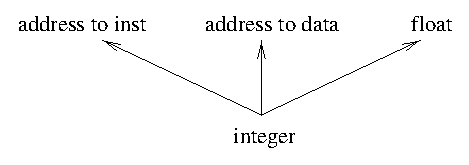
\includegraphics{figures/typeLattice.eps}}
\centerfigend{fig-typeLattice}{Lattice of Low-Level Types} 

Types are determined based on usage of a location across a live
range.  Given that a particular location can be re-used as 
different variables of different types by a compiler, the only
safe assumption is that the live range for a given location will 
have \emph{one} type.  {\emph{I believe this assumption is 
valid for non-overlapping registers.}} 

For the promotion of types, we use a slightly different lattice
to the one displayed in Figure~\ref{fig-typeLattice}.  Distinguishing
integers from addresses is a hard to solve problem as the assembly 
of the machine does not provide for mnemonic instructions to 
distinguish them.  For example, the following code: 
\begin{verbatim}
    sethi %hi(71167),%o1
    or %o1,%lo(71167),%o0
\end{verbatim}
sets register \texttt{\%o0} to the value of \texttt{71167}.  From 
looking at this code alone we cannot tell whether 71167 represents
an address (in the instruction or data area) or a large constant 
number.  Only usage of register \texttt{\%o0} will determine 
the type of 71167.  
For this reason we use the lattice in Figure~\ref{fig-promotionLattice} 
to describe the types of addresses; namely, an integer may ``look like'' 
and address, but until we can identify usage of that integer or 
address, we cannot determine whether it is an address (and hence 
promote to type address). 

\centerfigbegin
\resizebox{6cm}{!}{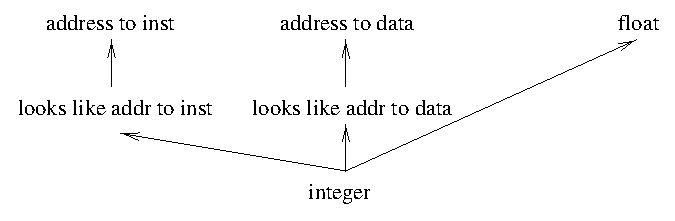
\includegraphics{figures/promotionLattice.eps}}
\centerfigend{fig-promotionLattice}{Lattice of Low-Level Types}

Once a type is determined, types are propagated across the live range 
of the particular location.

Note that even though we place data at the same memory locations
in the target address space as in the source address space, we 
still need to collect type information on pointers to data, as 
this information is needed in getting byte swapping (i.e. the 
simple endianness solution) to work correctly on translated 
programs.


\section{Type Analysis for Registers}
By default, a register is considered to be an integer 
register.  Usage of a register on a procedure call or 
as the return value of a call can change its type.  
Types are propagated from usage to definitions, so here are 
the steps to follow at different parts of the translation 
process: 

\begin{itemize}
\item Collect plausible type information at decoding time.
\item Perform type propagation by type induction.
\end{itemize}


\subsection{Collecting Type Information at Decode Time}
There are three rules that can be used at decoding time 
to annotate type information in registers.  

The first two rules deal with static checking of literal 
constants against addresses of text and data sections, and 
annotating the relevant register to ``looks like'' an address, 
denoted, ``\verb!~!pi'' for looks like a pointer to an instruction, 
and ``\verb!~!pd'' for looks like a pointer to data.  

\begin{typerule}
If a M$_S$-RTL instruction is of the form ``r = Num'' and 
$Num \in$ addrRanges(textSegments), then type(r) = \verb!~!pi.
\label{rule-llpi}
\end{typerule}

\begin{typerule}
If a M$_S$-RTL instruction is of the form ``r = Num'' and 
$Num \in$ addrRanges(dataSegments), then type(r) = \verb!~!pd.
\label{rule-llpd}
\end{typerule}

The following rule applies to any control transfer instruction, 
namely, calls, conditional and unconditional jumps. 
If the target address of the control transfer instruction is 
stored in a register, than that register has pointer to 
instruction type, denoted ``pi''. 

\begin{typerule}
If an M$_S$-RTL instruction is of the form ``controlTransfer r'', then 
type(r) = pi. 
\label{rule-pi}
\end{typerule}


\subsection{Determining Live Ranges of Registers}
In order to propagate types across registers and across 
procedures, live ranges for each register need to be found
first.  A register may take several different variables 
throughout the lifetime of a procedure, hence the need for 
such live ranges. 

A live range extends between the definition (i.e. assignment)
of a register until the death (i.e. re-assignment) of that register.
For example, in the following \texttt{main} code:
\begin{verbatim}
2    mov 10,%o0
3    mov 5,%o1
4    sethi %hi(.LLC0),%l0
5    call gcd
6    or %l0,%lo(.LLC0),%l0
7    mov %o0,%o3
8    mov %l0,%o0
9    mov 10,%o1
10   call printf
11   mov 5,%o2
12   ret
\end{verbatim}

The live ranges for register \texttt{\%o0} are: 
\begin{itemize}
\item Register \texttt{\%o0} becomes live at instruction 2,
    and its live range extends to instruction 5
\item instructions 5 to 8
\item instructions 8 to 10
\item instructions 10 to 12
\end{itemize}


\subsection{Propagating Type Information}
Type propagation can only be performed in \hrtl\ code, i.e. 
after parameter analysis recovery has been performed and 
the program's code has been lifted to the level of machine 
independent RTLs. 

Known types (i.e. non integer) are propagated across live 
ranges of registers, including across procedure calls, 
taking into consideration the signatures for library 
functions.

The first rule states how to go up the lattice when the type 
of the RHS is non integer, basically, propagate from the type of 
the usage to the type of the definition.

\begin{typerule}
If a \hrtl\ instruction is of the form ``r = exp'' and type(exp) = A 
and type(r) = int, then type(r) = A. 
\label{rule-prop-usageDef}
\end{typerule}
 
Note that the type of an expression is the type further up the
lattice of the individual registers forming the expression. 

The next rule looks at the return value of a function call 
and propagates that type to the newly defined register. 

\begin{typerule}
If a \hrtl\ instruction is of the form ``r = call X'' and 
returnType(X) = A, then type(r) = A. 
\label{rule-prop-retValue}
\end{typerule}

The next rule states that a library function's formal argument 
types are propagated to the associated actual parameters.  
In the case of variable argument functions, only the fixed 
formal parameter types can be propagated. 

\begin{typerule}
If a \hrtl\ instruction is of the form ``call libFunc(..., $r_i$, ...)'' 
and the function libFunc has the signature ``libFunc(..., $f_i$=$t_i$, ...), 
then type($r_i$) = $t_i$.  
\label{rule-prop-libFunc}
\end{typerule}
 
The above three rules can be applied on a pass through the code, 
without need of any extra data structures other than the live 
ranges for registers.  The next rule requires extra analysis to 
be performed on procedures, as a register that appears as 
pointing to an instruction may actually be invoked elsewhere in
the program, such as in the \texttt{qsort} program.  

\begin{typerule}
If there is an instruction of the form ``call r''and $\exists$ r2: 
type(r2) = \verb!~! pi, then, if r2 \ra* r, type(r2) = pi. 
\label{rule-reach}
\end{typerule}

In order to apply type rule~\ref{rule-reach}, we need to compute
the reaching definitions of $r2$ throughout the program, including
its transitive closure as the register could have been passed 
as parameter and then copied to another register before it is 
invoked. 


\section{Type Analysis for Other Memory Locations}
Type analysis of other memory locations
can be done to support endianness analysis:
the identification of when endianness swaps are necessary
when the target machine has a different endianness than the source machine.
A translated program's initialized memory is left as-is,
in the source machine's endianness.
We currently swap the bytes of \emph{every} multibyte value
that is read or written to memory.
If type analysis were extended
to include information about the endianness of each value,
then we could determine not only which endianness swaps are unnecessary,
but also when they must \emph{not} be done.
For example, the procedure \texttt{scanf}
is passed an address where its result must be stored.
The value that will be stored in memory
will be in native (target) endianness.
However, when the caller reads the value,
if its bytes are swapped, the native value will be corrupted.
This problem occurs today with every ``call-by-reference'' procedure
that takes addresses where their results are written.

We could do a data flow analysis to discover what values
have native endianness and what do not.
This could be done during type analysis
and a bit set indicating the endianness of each value and location.

Note that it is not enough to specify ``call-by-reference'' information
for just library procedures such as \texttt{scanf}.
The translated program's own procedures
may also be ``call-by-reference''. 


\section{Speculative Decoding}
Trees of program code can be built through speculative 
decoding, in such a way that a forest of trees is built, 
with the main tree being the one that starts at the 
program's entry point.  
Speculative decoding is useful if code ever gets code 
through the interpreter, in which case, the interpreter's 
switch manager can determine if the target address has
already been decoded, in which case, efficient translated
code is run instead of being interpreted.  However, 
speculative decoding is expensive on time resources, 
but for static translators this may be ok anyway.  
 
Type rule~\ref{rule-prologue} states that for all word-aligned
values of $N$ that belong to any of the text segments, if 
the first bytes of that address match a callee prologue (see  
Chapter~\ref{ch-call}, \S\ref{sec-callConvSpec} for SPARC and Pentium 
callee prologues), then $N$ is the start address of a new 
code tree.  

\begin{typerule}
$\forall N: N$ is word-aligned and $N \in addrRanges(textSegments)$ 
and $m[N] \ldots m[N+i]$ = callee\_prologue then type($L$) = $pi$.
\label{rule-prologue}
\end{typerule}

Clearly, applying this technique would be done after the 
normal decoding process and \uqbt\ should have tagged which 
word-aligned memory locations have already been processed 
so that those locations are ignored in this lengthy pass. 


\iffalse
\section{Promotion to Address to Data}
Addresses to data point to data locations in the program, such as
constant data (for example, strings that appeared in the original 
program), and global read and write data. 

An address is an integral number that happens to be a virtual address 
within the range of addresses of the data segment(s) of the program or of 
a symbolic name. 
In Elf binary-files, there are several sections that contain data; 
these are: 
\begin{itemize}
\item Sections that contain read-only data: .rodata, .rodata1
\item Sections that contain initialized read-write data: .data, .data1
\item Section of uninitialized read-write data: .bss
\end{itemize}
Each of these sections has identifying information to know the 
section name, its virtual address and its size.
This data provides us with information that can be used in 
determining whether an integer is an address to data or not. 

The following rules are used to promote integers to addresses to data.
We denote ``address to data'' by $addr_d$ and ``looks like address to 
data'' as $ll_{addr_d}$. 

\begin{typerule}
If $m[i]$ then type(i) = $addr_d$
\label{rule-index}
\end{typerule}

Type rule \ref{rule-index} states that any memory access implies an address 
through its index.  This will be the case for both load and store 
instructions.  Further, $i$ may be an expression, in which case 
the registers within it will contain the value of the address. 
For example:
\begin{verbatim}
  %o0 = m[%l0+4] 
\end{verbatim}
implies that \texttt{\%o0+4} is an address, in which case 
\texttt{\%o0} is the register that contains the address.  

\begin{typerule}
If $L_1 = a[L_2]$ then type($L_1) = addr_d$.
\label{rule-addressOf}
\end{typerule}

Type rule \ref{rule-addressOf} states that if the address of a location is 
taken, then the location represents an address to data.  For example,
the following two RTLs illustrate this point:
\begin{verbatim}
  r[24] = a[m[0x804a250]]
  r[24] = a[m[r[29]-8]]
\end{verbatim}

\begin{typerule}
If $L = Num$ and $Num \in$ addrRange(dataSegments) then type($Num) = ll_addr_d$ 
and type($L) = ll_{addr_d}$.
\label{rule-dataSeg}
\end{typerule}

Type rule \ref{rule-dataSeg} states that if an integral constant is within 
the range of the virtual addresses of the data segment(s) of a program (i.e. 
.rodata, .rodata1, .data, .data1 or .bss in an Elf binary-file), then 
both the integral constant and the location to which it is assigned 
looks like an address to data.  

\emph{Is the information in the dynamic symbol table for type STT\_OBJECT 
relevant?  It contains the virtual address of such objects.}

As can be seen, the type rules that promote to address to data cannot
always solve the problem of accessing data addresses.  However, in 
our implementation, we \emph{force} the data segment(s) of the source 
binary program to be located at the same virtual addresses in the
target program.  Hence, determining whether an address points to 
data or not, does not need to be solved using this model; and 
type rules~\ref{rule-index} to \ref{rule-dataSeg} are not used. 


\section{Promotion to Address to Instruction}
An instruction address points to instructions in a program, normally
the start of procedures or entry points into the code of a function. 

An address to an instruction is a virtual address that falls 
within the text section(s) of the program.  For Elf binaries, the
following sections contain instructions: 
\begin{itemize}
\item The program's text section: .text
\item The program's initialization section: .init
\item The program's finalization section: .fini
\item The program's program linkage table: .plt
\end{itemize}
Further, the dynamic symbol table (.dynsym) also contains names of 
dynamic library procedures.  Such names map addresses which are 
found in the PLT section.

The following rules are used to promote integers to addresses to 
instructions.  We denote ``address to instruction'' by $addr_i$ 
and ``looks like an address to instruction'' by $ll_{addr_i}$.

\begin{typerule}
If $Call L$ then type($L$) = $addr_i$.
\label{rule-call}
\end{typerule}

Type rule \ref{rule-call} states that if a call is made to a target 
location, then that location represents an address to an instruction. 
This rule covers both, calls to known addresses and otherwise, 
such as in the following examples: 
\begin{verbatim}
  call 0x10ae4        ; known target address
  call r[10]          ; computed call, unknown statically unless analyzed
\end{verbatim}

\begin{typerule}
If $Jump L$ then type($L$) = $addr_i$.
\label{rule-jump}
\end{typerule}

Type rule \ref{rule-jump} states that the target location of an 
unconditional jump points to an instruction.

\begin{typerule}
If $Jcond L$ then type($L$) = $addr_i$.
\label{rule-jcond}
\end{typerule}

Type rule \ref{rule-jcond} states that the target location of a 
conditional jump is an address to an instruction.

\begin{typerule}
If $L = Num$ and $num \in$ addrRange(textSegments) then 
type($Num$) = $ll_{addr_i}$ and type($L$) = $ll_{addr_i}$.
\label{rule-textSeg}
\end{typerule}

Type rule \ref{rule-textSeg} states that an integral constant looks 
like an address to an instruction if that constant is within the
range of virtual addresses of the text sections of the program. 
In the case of Elf binary-files, the text sections are .text, 
.init, .fini and .plt. 

\begin{typerule}
If type($L$) = $ll_{addr_i}$ and $L$ uniquely reaches $r[i]$ in 
a $Call r[i]$ statement, then type($L$) = $addr_i$.
\label{rule-reach2}
\end{typerule}

Type rule \ref{rule-reach2} states that a reaching definition of a 
location that looks like an address to an instruction is in fact
an address to an instruction, if the statement it reaches is a 
computed call on a register.

\begin{typerule}
If type($L$) = $ll_{addr_i}$ and $m[L] \ldots m[L+n]$ = callee\_prologue
then type($L$) = $addr_i$.
\label{rule-prologue}
\end{typerule}

Type rule \ref{rule-prologue} states that an integral constant that 
looks like an address to instructions can be promoted to an 
address to instruction if the bytes at that memory location and subsequent 
locations match those of a valid callee prologue (see 
\S\ref{sec-callConvSpec} for SPARC and Pentium callee prologues).

Type rule \ref{rule-prologue} creates a forest of code that is decoded
statically, even when the caller of such code cannot be determined
statically.  In the event of dynamic invocation of such code, 
if the code has been translated, the interpreter's switch manager
will check the address translation table and determine that such
code has already been translated, hence giving control to it 
instead of interpreting it. 

By the nature of building the control flow graph while decoding 
machine instructions, we are in essence applying type rules~\ref{rule-call} 
to \ref{rule-jcond}.  

Type rules~\ref{rule-textSeg} promotes a type to ``looks like an 
address''.  If neither type rules~\ref{rule-reach2} or~\ref{rule-prologue} 
applies, then we cannot say that the particular integral constant is an 
address or not.  As it \emph{may} be an address, we will need to 
pass it as an address in order to prevent programs from crashing. 
In the event that it was an integral constant instead of an address, 
we will emit the wrong result.  

\emph{Can we somehow trap this?  If it goes to a library function,
we have the signature in most cases (except varargs), if it goes 
to user code, then we would have translated it, so we could check 
prior to invoking?}
 

\section{Promotion to Float Type}
A float type is determined when placing a location onto a 
floating point register.  Type conversion procedures such as 
\texttt{itof()}, integer to float, not only perform a type 
conversion but also set the live range of the source and 
target registers used; the source register dies and the target
register starts its live range.  The size of a float is determined
based on the usage of the floating point register(s).  For 
example, when a double register is used, then its size is twice 
the word size (64 for SPARC). 

There are two different types of float values, those that are 
constant and those that go into registers.  The constant values
are easy to determine from the RTLs, as a float number is 
represented by \texttt{FloatNum} in the EBNF and an integer 
number as \texttt{Num}.  

Floating point registers are separate to integer registers in our
RTL model, hence any values that pass through floating point 
registers are of type float.  Further, floating point operators 
and procedures (such as sin and cos) also aid in determining how a 
particular register is used.  

The following rules determine the values of type float: 

\begin{typerule}
If $V = FloatNum$ then type(V) = float.
\label{rule-float}
\end{typerule}

Type rule~\ref{rule-float} states that if a value is of the 
RTL type FloatNum, then it is a floating point value.

\begin{typerule}
If $L = FFunction$ then type(L) = float.
\label{rule-floatFunc}
\end{typerule}

Type rule~\ref{rule-floatFunc} states that if a function that
returns a float is used, then the type of the location becomes
a float.
Note that this rule implies that a register may be used to 
hold integer and floating point values at different points in 
time in the program, hence the live range for a register needs 
to be considered carefully. 

\begin{typerule}
If $L = (Exp BinOP Exp)$ and $BinOP \in Farith$ then type(L) = float.
\label{rule-floatOp}
\end{typerule}

Type rule~\ref{rule-floatOp} states that if a floating point arithmetic
operand is used on the right-hand side expression being assigned to 
location $L$, then the result type of the expression is a float and
hence $L$ is of type float.

\fi


\section{Register Live Ranges}
In order to perform some of the promotion analysis, we need to 
keep track of live ranges for all registers used in a procedure. 
The importance of this is that a register may hold values of 
different types at different points in the program, hence we 
cannot just say ``register 5 is of type float'' as it may be
that it is of type integer and then becomes of type float.  
\emph{A suitable data structure to keep track of ranges and 
types is needed.}

\emph{The following example should be on the RTLs rather than
the assembly code, but uqbts is giving the wrong answer}

A live range extends between the definition (i.e. assignment) 
to a register until the dead (i.e. re-assignment) of that register. 
For example, in the following \texttt{main} code from Figure~\ref{fig-c_gcd}: 
\begin{verbatim}
2    mov 10,%o0
3    mov 5,%o1
4    sethi %hi(.LLC0),%l0
5    call gcd  
6    or %l0,%lo(.LLC0),%l0
7    mov %o0,%o3
8    mov %l0,%o0
9    mov 10,%o1
10   call printf  
11   mov 5,%o2
12   ret
\end{verbatim}

By the time the analysis is done, we will have performed the 
prologue/epilogue analysis, hence the first and last instructions 
are not there.  The live ranges for register \texttt{\%o0} are: 
\begin{itemize}
\item Register \texttt{\%o0} becomes live at instruction 2, 
	and its live range extends to instruction 5 
\item instructions 5 to 8 
\item instructions 8 to 10
\item instructions 10 to 12
\end{itemize}


\section{Reaching Definitions}
In order to apply type rule~\ref{rule-reach}, we need to compute 
the reaching definitions of $L$, the transitive closure of 
reaching definitions.  The use of the \texttt{qsort} example 
is ideal in this case, as two levels of indirection are needed 
in order to find the location where a function pointer gets used. 


\section{Type Recovery Analysis Implementation}

{\small
\begin{flushright}
Implementation and documentation: Bernard [Aug 01]
\end{flushright}
}

In order to evaluate the type recovery processes discussed in the previous
sections of this paper, an initial implementation of type recovery
analysis based on this paper has been completed.

This implementation however is only an initial version and does not
implement every rule stated in this paper. The following is a list of 
type rules that the current version of type recovery analysis implements:

\begin{itemize}
\item Type Rule~\ref{rule-pi} "controlTransfer r", then type(r) = pi
\item Type Rule~\ref{rule-prop-usageDef} "r = exp" and type(exp) = A and 
	type(r) = int, then type(r) = A
\item Type Rule~\ref{rule-prop-retValue} "r = call X" and returnType(X) = A 
	then type(r) = A
\item Type Rule~\ref{rule-prop-libFunc} Type propagation between library 
	functions
\end{itemize}

Without rules~\ref{rule-llpi} and \ref{rule-llpd}, it is not possible to 
implement the ``looks like'' types mentioned earlier in this paper.  
Therefore, the different low-level types that are represented are integer, 
address to instruction, address to data and float.

The first necessary step is to infer the plausible type information of each 
register in each of its live ranges. This step is done after the binary
files has been brought up to the HRTL level of abstraction. It is possible
to perform the initial type recover at the machine specific RTL level. However,
important information such as parameters and return value to functions are not 
available at the machine specific RTL level and will need to be added later. 
For simplicity of implementation reason, it was decided that the type recovery 
analysis will begin after the binary file has been bought up to the HRTL level.

The first information that we want to gather from the HRTL is the location
of every use and definition of each register. From this information, we
can build use-definition chains and determine the live ranges of each register.
Since we assume that the type information for a non-overlapping register in a 
particular live range is always the same, therefore each use-definition chain 
would only have one type and can be used as a means to propagate type 
information of each register across instructions. The use-definition chain 
is therefore one of the most important data structure we use for type recover.

To actually infer the type information, the HRTL instructions need to be parsed
for specific cases that uncover the type information. The HRTL instructions are 
stored in a prefix format as a list of integers called semantic strings. The 
simplicity of this prefix format allowed the creation of a parser, specific
to uncovering type information from semantic strings, to be a relatively 
straight forward process. The following is a list of some of the cases
which the parser is looking for:

\begin{itemize}
\item Registers within MemOf tokens. This can be complicated by functions
	and operations following MemOf tokens.
\item Registers following a control transfer token. 
\item Certain binary operator that has implict type information to the registers
	it operates on.
\item Certain function operators, which often has explict type information
	to the registers it operates on.
\end{itemize}

The parser will first find all the registers that are in the semantic string and
determine whether it is a use or definition of the register. It will insert
this information into a use-definition chain data structure. The parser will
also insert into the data structure any type information that it can infer.

Additional, the parser will look for simple register aliasing situations that 
can later be used for type propagation. For example, in the following example, 
register 1 and register 2 are consider aliases in type value. The 
use-definition chains of these two register at this particular point will be 
linked together. Therefore, if more type information was later discovered 
about register 2, the type information of register 1 would also be updated.

\begin{verbatim}
r[1] = r[2]
\end{verbatim}

This stage of type recovery will already uncover a significant amount of type
information. Long use-definition chains will likely have the correct type
information as the many uses of the register would most likely uncover the
type. 

In order to find the complete use-definition chains for every register, the
program must be analyzed in its entireity. Each register must be tracked 
from its first definition to its last use. There are several implementation
problems with tracking a register in that manner. One problem is the difficulty
in tracking a register as the flow of instruction passes a control transfer
instruction. A register can be defined before the control transfer instruction 
and then be used in both the branches. Therefore, the data structure used for 
the use-definition chains must be complex enough to handle this case correctly.
A second problem is the size of the data-structure used to hold the 
use-definition chains. Since the backend of UQBT that performs code generation 
only looks at HRTL code a basic block at a time, it would be much more 
convenient to also have use-definition data structures for each basic block 
instead of a monolithic one for the whole program. 

The approached that was taken in this implemenation was to create use-definition
chains at the basic block level. This was chosen mostly because of its 
simplicity.  The use-definition chains will always be straight lines at the 
basic block level, as there will not be any control transfer instructions. 
Retrieving the information to insert into the data-structure is also a simple 
process as all the information can be found inside each basic block. 
Therefore, the code to generate the data structure is small and modularized 
for different types of basic blocks. However, the main disadvantage to creating
the use-definition chains at the basic block level is that the chains are 
often incomplete. Many chains will only have uses but no definitions and some 
chains will only have definitions but no uses.
Therefore, this data structure does not store the equivalent amount of 
information as the one that covers the complete program. However, the missing 
information can be recovered by performing type propagation across basic 
blocks and across functions.
The type propagation is simply completing incomplete chains across basic 
blocks and functions. 

To implement type propagation across basic blocks, a depth first traversal of 
the basic blocks inside each function is performed. During the depth first 
traversal, a pointer to the parent of each basic block is kept inside the 
basic block's data structure. At each basic block, use-definitions chains that 
have uses but no definitions are found and are made candidates for type 
propagation. Determining which chains are candidates is a very quick task as 
there are only certain places where incomplete chains may be. Incomplete 
chains are always found as the first use-definition chain of each register.
And each chain can only have one definition which, if it exists, is always 
the first element in the chain. Therefore, only $n$ elements needs to be looked 
at for each basic block to determine which chains need to be propagate, where 
$n$ is the number of registers. Next, to find the definition part of the 
chains, the algorthm will traverse up the call graph, using the pointer to 
the parent basic block stored during the traversal. 

Since this traversal follows the flow of normal execution, traversing back up 
the control flow graph should always find the desired register definition. 
However, there are cases where this might not be true because of the 
limitation of keeping only one single pointer to the parent basic block. It 
also depends on the aggressiveness of the traversal.

The original traversal algorithm that was implemented would only consider every
basic block once. Once a particular basic block has been reached, a flag is 
marked to indicate that future traversals should end before reaching this basic
block. However, this traversal is much too conservative as it only consider one
path to each basic block when there could possibly be many paths. To solve this 
problem, a more aggressive traversal algorithm allowed a basic block to be 
traversed multipled times. To avoid infinite loops, it still marks basic blocks
that have been traversed. When a basic block that has been traversed is reached,
it would be traversed again but be treated as a leaf node. Therefore, the 
algorithm would not continue to traverse down this path any further and avoid 
possible infinite loops. However, this still introduces a possible infinite 
loop situation when dealing with back branches due to the limitation of 
keeping only one pointer to the parent's basic block. 

\begin{verbatim}
   A
   |
   B      Assume the straight path from B to C is going down
   |\     and the crooked path from B to C is goind up (back branch)
   |/
   C
\end{verbatim}   
	  
Suppose that register 1 is defined in basic block A and used in basic block 
B. To traverse this graph, the path A-B-C would be taken. Once basic
block C has been reached, it would try to traverse to basic block B. Since
basic block B has already been traversed before, its traversal flag will 
be set. However, with the second algorithm, it would still be traversed
again and treated as a leaf. 

When basic block B is reached for the second time, it is discovered that
it contains a use-definition chain with uses but no defines for register 1.
Backwards traversal of the graph using the parent pointer would be used to
find the basic block with the definition of register 1. However, the parent
pointer of basic block B now points to basic block C, and the parent pointer
to basic block C points to basic block B. Therefore, this traversal will never
complete as the definition of register 1 is in basic block A.

To work around this possible problem, the implemented algorithm will try to 
detect any loops in the traversal. In most cases, this is enough to overcome 
this problem. However, there still exist cases where infinite loops can occur. 
A maximum number of basic block traversal was added to work around these 
special cases.

Propagating type information across functions is done in a very similar way as
propagating across basic blocks. The complexity of propagating across functions
is slightly higher as every call site and every return site in each function
must be recorded. With propagation of return value, it could involve a large set
of registers as a function can have many return sites which would all involve
different use-definitions chains of registers. This is actually benefitual to
the type propagation as it implies that the whole set of registers must all 
be the same type.

Type propagation may seem to be even more complicated and complex than simply
creating complete use-definition chains. However, the beauty of type 
propagation is the ability to propagate type information from library 
functions. Since the type information for parameters and return value for 
standard C functions are known, any call to these functions will allow 
trusted type information to be propagated back to user functions.


\subsection{Results}
The following type information was inferred for the function \texttt{myCompare}
which can be found in the \texttt{qsort2} regression program:

\begin{verbatim}
Currently In Procedure: myCompare
Registers stored in this Basic Block are:
8       --> Def @ 108c8    -->  <32pd>  Use @ 108cc 99
                                        Contains Alias
        --> Def @ 108cc    -->  <32i>   <no_use>
9       --> Def @ 108cc    -->  <32pd>  Use @ 108cc 99
                                        Contains Alias
24      --> Def @ param    -->  <32pd>  Use @ 108c8 0
                                        Contains Alias
25      --> Def @ param    -->  <32pd>  Use @ 108cc 0
                                        Contains Alias
\end{verbatim}

The above data output shows that we were able to identify that register 8 was
defined at address 108c8 and used at address 108cc. It also identified that
the register is of pointer to data type at those two instructions. Registers 24
and 25 were also identifed to be pointers to data. The information about
registers 24 and 25 is especially important as both these registers are 
parameters to the myCompare function. Therefore, we now know what the type 
signature for the myCompare function is. Also, all the register shown above
contain aliases. Therefore, if we found out any new type information about one
of these registers, the type information of at least another register would
also be updated.

This type information was manually checked against the HRTL instructions and 
also the original source code and was verified to be correct. However, no 
automated testing system to determine the type information correctness is 
currently available.


\subsection{Future work}
There are several areas which need to be worked on in order for more accurate
type recovery analysis in the future. Currently, although the type information 
for most registers are recovered, there still exist cases where the type 
information for a register is still not available. For these cases, 
rules~\ref{rule-llpi} and \ref{rule-llpd} can be used to determine possible 
type information. These possible type information may not be always correct 
but would allow the backend additional information to determine what the 
correct code that it needs to generate.

Type analysis should be extended
to determine the endianness of each value and location.
This is needed to know when it is incorrect to swap the bytes
of values loaded or stored to memory.
It will also allow us to avoid doing swaps that are unnecessary.

Backend support of the type analysis recover will also need to be added in the 
future. The information gathered through type analysis should significantly 
increase the correctness of the code generated by the backend.

Finally, a test suite that can automatically verify that the inferred type 
information is correct needs to be written. Currently, the only method of 
verification is manually analyzing every HRTL instruction by hand. An 
automated method that can use the orginal C source code to verify type 
information would be the ideal tool.

The current implementation has not been thoroughly tested, some 
propagation across procedures is not working as expected. 


